%! TEX root = ../thesis_main_sample.tex

\chapter{体裁ガイドライン}
	\label{chp:guideline}

	本文書は、東京大学教育学研究科生涯学習基盤経営コース及び同教育学部教育実践政策学コースの所属学生が執筆する学位論文の執筆スタイルを規定するものである。
	以下、断りが無ければ「本コース」を上記2コースの総称とする。
	本章でスタイルの詳細について記述し、次章では本文書の生成に用いたテンプレートファイルについて述べる。

	\section{言語}
		\label{sub:language}

		執筆に用いる言語は日本語または英語とする。
		ただし、教育学研究科修士論文要旨及び教育学部卒業論文要旨は必ず日本語で書くことになっている。
		以下、本節で説明するスタイルは日本語での執筆を対象とする。
		英語で執筆する際は、研究対象の領域に最も近い学術雑誌のスタイルガイドを選び、準拠すること。
		その際、準拠したスタイルガイドは学位論文中に明記せよ。

	\section{製本上の構成}
		\label{sub:seihon}

		本コースの学位論文はA4用紙に印刷し、左綴じで製本のうえ提出すること。
		このとき枚数が少なすぎると安定しないので,100ページ以内であれば片面印刷するとよい。
		その他、本コースにおける製本の規定及び実践的なアドバイスについては\cref{app:seihon}で案内があるので参照されたい。
		学位論文の中身は次の順番で製本すること。

	\begin{itemize}
		\item 表題紙
		\item 目次
		\item 本文
	\end{itemize}

	以上の構成要素の詳細については\cref{sec:layout}以下を見よ。
	卒業論文は本文が20枚以上であることが要件である
	\footnote{修士論文には枚数規定はない。}。

	\section{全体のレイアウトと字体}
		\label{sec:layout}

		以下はテンプレートを適切に利用すれば自動的に適用される。

		\subsection{レイアウト}
			\label{sub:layout}

			\subsubsection{表題紙}
				\label{subs:titlepage}

				提出年度と学位論文の種類(修士論文または卒業論文)を上余白40mm以上とって配置し、そこから45mm程度を空けて論文題目(サブタイトル含む)を置くこと。
				下余白30mm程度の位置に、自身の所属(大学・大学院名、学部・研究科名、学科・専攻名、コース名)、学籍番号、氏名、指導教員名・職名を記述せよ。
				文字は全て中央揃えとする。
				表題紙にはページ番号を振らない。

			\subsubsection{目次}
				\label{subs:tableof}

				表題紙に続けて、本文の章節目次を作成する。
				目次タイトルと目次本体があれば、後者のレイアウトは1段組である限りにおいて自由とする。
				図表を含むときは図目次、表目次の順に追記するようにせよ。
				このとき、各目次は改ページしたうえで連結すること。
				また、目次にはローマ数字(i, ii, iii, \dots)など本文と異なる数字を用いて独自のページ番号を振るようにする。
				ページ番号の場所は本文(\cref{subs:body})に同じ。

			\subsubsection{本文}
				\label{subs:body}

				本文は1段組で構成し、文字数は1行45字程度、行数は35行程度とする。
				余白は左右25mm、上下30mm程度をとること。
				ヘッダーとフッターを考慮しても、本文と上下の余白が40mm以上離れていればよい。
				本文が100ページを超えて両面印刷にて製本する場合、奇数ページ・偶数ページごとに左右の余白を変えてもよい。

				\paragraph{ヘッダー・フッター}
					\label{subs:header_footer}

					フッター中央にはページ番号のみを配置し、原則としてヘッダーには何も書かないものとする。
					各節が十分に長いために読者が道に迷う可能性があるとの懸念にしたがって、可読性のために章節タイトルを表示するなどの運用は可とする。


		\subsection{書体・書式・文字サイズ}
			\label{sub:font}

			本コースの学位論文の、文字から構成される要素は\cref{tab:font}に示す書体・書式・文字サイズを用いよ。
			ただし、表題紙について、年度と学位論文の種類は項タイトル、
			所属・指導教員・学籍番号・氏名・指導教員は本文と同じとする。
			また、小項以下の項目立てを用いる場合には項タイトルと同じくし、頭に記号を用いるなどして項タイトルと差異化せよ。

			\begin{table}[tb]
				\caption{文字から構成される論文上の要素に用いるべき書体・書式・文字サイズ}
				\label{tab:font}
				\centering

				\begin{tabular}{lccc}
				\toprule
				\textbf{構成要素} & \textbf{書体} & \textbf{書式} & \textbf{文字サイズ}\\
				\midrule
					論文題目 & 明朝体 & 立体 & 18pt \\
					サブタイトル & 明朝体 & 立体 & 14pt \\
					章タイトル & ゴシック体 & 太字 & 20pt \\
					節タイトル & ゴシック体 & 太字 & 14pt \\
					項タイトル & ゴシック体 & 太字 & 12pt \\
					本文 & 明朝体 & 立体 & 20pt \\
				\bottomrule
				\end{tabular}
			\end{table}

	\section{本文の構造化方法}
		\label{sec:structure}

		本文の構造は以下の順とする。

		\begin{enumerate}
			\item 各章(注は脚注として内包)
			\item 謝辞
			\item 参考文献
			\item 付録
		\end{enumerate}

		各章の内部は、論理的に章・節・項の3階層に収まるのが構成のわかりやすさと読みやすさの観点から望ましい。
		節・項の番号付けはハーバード方式(2.3.1のような形式)とする。
		小項以下は箇条書きなどで適宜代用し、目次への記号の反映は任意とする。

		付録と謝辞は章と同等の扱いとするが、付録にはアルファベット大文字で「付録A」などと番号付けする一方、謝辞には章番号をつけないものとする。
		参考文献の詳細はあとで述べる。

	\section{本文の表記方法}
		\label{sec:writing_manner}

		\paragraph{句読点}
			\label{par:punct}

			和文は句点を全角コンマ(,),読点を全角読点(。)とする。
			欧文中では半角のコンマ (,)とピリオド (.) を用い、半角スペースを後置する。
			また和文中に欧文の句を挿入する際には、半角スペース相当の空白を入れること
			\footnote{WordでもLaTeXでも自動で入る。}。

		\paragraph{強調}
			\label{par:inline_markup}

			文章の一部、単語や句を強調したい場合、和文には\emph{太字}のみを用い、斜体は使わないようにせよ。
			このとき太字はゴシック体にするのが望ましいが,統一されている限りにおいて明朝体でもよい。
			読みにくくなるため、引用文で用いられている以外は下線,圏点の利用は控える。

			一方、欧文の強調はセリフ体の斜体を基本的に用いることとし,太字・ゴシック・下線の利用は控える。
			ただし、強調したい和文キーワードの一部に欧文が含まれる場合は、和文と揃えて太字にする(例:\textbf{MARCフォーマット})。

			以上において控えるべきとした強調方法については、強調部分のなかでさらにその一部を強調したい場合であれば利用してよいものとする。

		\paragraph{図表}
			\label{par:fig_tab}

			図表は任意の位置に置いてよいが、図表番号及びキャプションを必ず付与すること。
			ただしその位置は、表については上に、図については下に付与するものとする(e.g., \cref{tab:font,fig:sample})。
			図表番号はハーバード方式に従っても、全体を通して連番としてもよい(本要綱では前者とした)。

			\begin{figure}[tb]
				\centering
				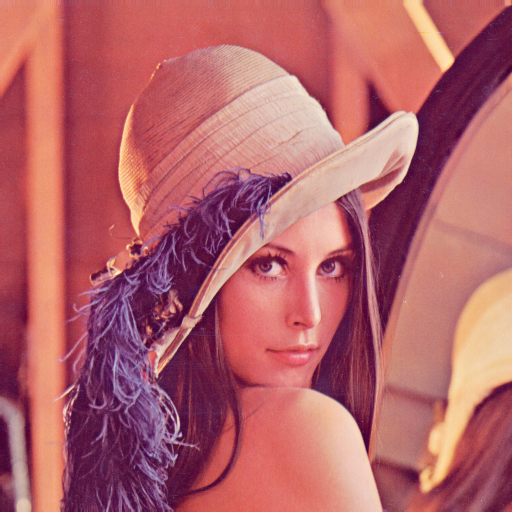
\includegraphics[width=5cm]{figure/Lenna.png}
				\caption{サンプル画像として著名な Lenna Sjööblom さん}
				\label{fig:sample}
			\end{figure}

		\paragraph{記号}
			\label{par:symbol}

			本文中でよく使われる一方で誤用の多い記号類について注意点を述べる。

			\begin{description}
				\item[二重かぎかっこ(『, 』)] 和文書籍の書名を表すときに用いよ。英語と違って太字にしないこと。
				\item[丸かっこ((, ))] 欧文中で丸かっこを使うときはその前後にスペースを入れることに注意せよ。また、和文を内包させる場合は全角にする。
			\end{description}

			\noindent
			その他、とくに欧文(英語)環境における正しい記号の使い方は \texttt{english punctuation} などのキーワードでweb検索するとよい。

		\paragraph{引用}
			\label{par:cite}

			参考文献の一部を文字通り引用する場合、本文中に埋め込む方式(inline quote)とパラグラフとして分離する方式(block quote)の2つがある。
			inline quote であるが、次に示すようにかぎかっこ(「, 」)で引用部分を囲み、文中に埋め込めばよい。
			ただし引用文中にもかぎかっこがある場合は、二重かぎかっこ(『, 』)に変更すること
			\footnote{引用文がさらに2重かぎかっこを含む場合はかぎかっこに変更する。}。

			\begin{itembox}[l]{Inline quote}
				澤田昭夫は良い論文について \textcquote[p. 19]{sawada}{よい論文は統一unity,連関coherence,展開developmentにおいて優れた論文あるいは明確性clarityにおいて優れた論文}だとしている。
			\end{itembox}

			\noindent
			次に block quote であるが、次のように前後と左側に余白を与えるようにする。
			3行以上になるようであれば block quote を使うようにするとよい。

			\begin{displaycquote}[p. 74]{sawada}
				論文書きでもっとも大切なのは,問を疑問文の形で切り出すことで,それがレトリックで言う発見・構想です。
				もっとも大切だというのは,それができればつまり全体を貫く主な問が何であるかを確定することができれば,論文の首尾一貫性,統一性を保証する基本的条件が整ったことになるからです。

				そのつぎに大切なのは,論文の構成,材料の配置です。
				その際,肝に銘じなければならないのは,構成・配置の大原則は起承転結ではなく,序・本・結(序と本論と結び)だということです。
			\end{displaycquote}

			\noindent
			いずれも引用元の参考文献と、当該引用文が記載された箇所(ページ番号など)を引用の末尾に明示すること。
			その記述方法は\cref{sub:ref_style}と同様である。


	\section{参考文献スタイル}
		\label{sec:bib_style}

		本説では、本文中で参考文献を示すときの参照方法と文献リストの記述法を述べる。

		\subsection{参照方法}
			\label{sub:ref_style}

			基本的には主語として「著者 (年)」とするか、文末に「(著者, 年)」を置く \emph{author-year} 形式が望ましいが、一貫している限りにおいて \emph{number} 形式(参考文献に番号を振り、「[1]」のように参照する)も可とする。

		\subsection{文献リストの記述方法}
			\label{sub:ref_list_sylte}

			基本的には、本項で紹介するスタイルを採用せよ。
			ただし論文全編にわたって一貫している限りにおいて、各自の研究領域に最も近いスタイルを使っても良い
			\footnote{例えば本テンプレートの参考文献リストは日本経済学会に準拠している。}。
			その際は指導教員やその指導を受けている先輩の院生に確認すること。
			リストに記載する文献の順番は「著者順」または「(本文での)引用順」のいずれかとする。

			% 参考文献リストの書式の乱れは研究姿勢の乱れであることを自覚するように

		\subsubsection{図書の場合}

			\begin{description}
				\item[和:] 著編者名 『書名』 \{版表示,\} \{出版地,\} 出版社, 出版年, \{総ページ数,\} 当該部分のページ.
				\item[洋:] author. \textit{title}. \{edition,\} place of publication, publisher, year, \{total page,\} page.
			\end{description}

			\begin{screen} \begin{itemize}
				\item 近藤二郎 『社会科学のための数学入門』 東京経済新報社, 1973,
				p. 37--40.

				\item Barzun, Jacques and Graff, H. F. \textit{The Modern Researcher.}
				Rev. ed., \\New York, Harcourt, 1970, p. 165.
			\end{itemize} \end{screen}


		\subsubsection{翻訳書の場合}

			\begin{description}
				\item[和:] 著編者名 『書名』[原書名(イタリックで記載) \{版表示,\}
				\{出版地, \} 出版社, 出版年,] 翻訳者名, 出版社, 出版年, \{総ページ数,\} 当該部分のページ.
				\item[洋:] author. \textit{title of translation} [\textit{original title}. \{edition,\} place of publication, publisher, year,] name of translator, place of publication, publisher, year, \{total page,\} page.
			\end{description}

			\begin{screen} \begin{itemize}
				\item Varles, Jana ed. 『情報の要求と探索』 [\textit{Information Seeking:
				 Basing Services on User's Behaviors.} North Calolina,
				 McFarland \& Company, 1987] 池谷のぞみ,	 市古健次, 白石英理子, 田村俊作訳,
				 勁草書房, 1993, p. 10.

				\item Schneider, Georg. \textit{Theory and History of Bibliography.}
				 [\textit{Handbuch der Bibliographie.} e Aufl., Berlin, Knopt, 1978,]
				 tr. by R. R. Shaw, New York, Columbia University Press, 1934, p. 14--15.
			\end{itemize} \end{screen}

		\subsubsection{編集書の一部(図書形態の論文集の一論文を含む)の場合}

			\begin{description}
				\item[和:] 当該部分の執筆者名 ``当該部分の題名'' $<$編者名 『書名』 \{版表示,\} \{出版地,\} 出版社, 出版年$>$ \{総ページ数,\} 当該部分のページ.
				\item[洋:] author. ``\textit{title}''. $<$editor. \textit{book title}, \{edition,\} place of publication, publisher, year$>$ \{total page,\} page.
			\end{description}

			\begin{screen} \begin{itemize}
				\item 宮坂広作 ``余暇と社会教育'' $<$碓井正久編著 『社会教育』 第一法規, 1970$>$ p. 201--203.

				\item Groom, Geofrey. ``Bibliography of older material'' $<$Garvin, L. H. ed. \textit{Printed Reference Material.} 2nd ed., London, Library Association, 1984$>$ p. 456--501.
			\end{itemize} \end{screen}


		\subsubsection{逐次刊行物掲載記事(雑誌論文を含む)の場合}

			\begin{description}
				\item[和:] 執筆者名 ``論題名'' 『掲載逐次刊行物名』 vol. XX, \{no. XX,\} 発行年\{月\}, 当該部分のページ.
				\item[洋:] author. ``\textit{title},'' \textit{name of periodical}, vol. XX, \{no. xx,\} year\{month\}, page.
			\end{description}

			\begin{screen} \begin{itemize}
				\item 小野寺夏生 ```Bibliostatistics': 情報現象の統計学的説明'' 『情報管理』
				vol. 21, no. 10, 1979, p. 782--802.

				\item 小野寺夏生, 中井浩 ``単純なモデルからのZipfの法則の導入'' 『情報科学技術
				研究集会論文集』 vol. 33, no. 3, 1977, p. 129--138.

				\item Brookes, Bertram C. ``Theory of the Bradford Laws,'' \textit{Journal of
				Documentation,} vol. 33, no. 3, 1977, p. 180--209.

				\item Nelson, Micheal J. and Tague, Jean M. ``Sprit Size-Rank Models for the
				Distribution of Index Terms,'' \textit{Journal of the American Society
				for Information Science,} vol. 36, no. 5, 1985, p. 283--296.
			\end{itemize} \end{screen}

		\subsubsection{Web上のリソース}

			web上のリソースについては,書誌情報の最後に ``入手先URL (アクセス日)''
			(``available from (URI), (accessed date)'') を記入する。
			それ以外の項目は図書並びに逐次刊行物掲載記事の規定に準じ,入手先の情報から明らかである項目を記述せよ。

			\begin{screen}
				 情報メディア学会 ``『情報メディア研究』への各種原稿の投稿について'' http://www.jsims.jp/toko.html (アクセス日: 2008/10/27)
			\end{screen}
